\documentclass{article}
\usepackage[utf8]{inputenc}
\usepackage{amsmath,amssymb,amsfonts}
\usepackage{graphicx}
\usepackage{hyperref}
\usepackage{geometry}
\usepackage{algorithm}
\usepackage{algorithmic}
\geometry{a4paper, margin=1in}
\usepackage[english,russian]{babel}

\usepackage{listings}
\usepackage{xcolor}
\usepackage[utf8]{inputenc}
\lstset{
  language=Python,
  basicstyle=\ttfamily,
  breaklines=true,
  numbers=left,
  numberstyle=\tiny,
  keywordstyle=\color{blue},
  commentstyle=\color{green},
  stringstyle=\color{red}
}


\begin{document}

\title{методы отбора признаков, индекс Gini}
\author{}
\date{}
\maketitle

\section*{Введение}
В задачах машинного обучения часто не сразу понятно, какие признаки реально важны для построения модели. В итоге в данных может оказаться много лишнего шума, который только мешает. "Шумовые" признаки снижают качество модели и увеличивают время её работы. Поэтому перед тем, как приступить к обучению модели для классификации, регрессии или прогнозирования, важно отобрать наиболее информативные признаки.

Хороший отбор признаков зачастую важнее, чем ускорение обработки данных или небольшое повышение точности модели. Например, в медицине минимальный набор значимых признаков может быть ключевым для создания эффективного диагностического теста.

\section*{Индекс Gini}
Индекс Gini вычисляется для каждого признака и для всех возможных пороговых значений. Он определяется как вероятность того, что два случайно выбранных образца из набора данных будут иметь разные классы. Чем ниже индекс Gini, тем лучше признак разделяет классы.

\subsection*{Вычисление}

Численно коэффициент равен площади фигуры, образованной линией абсолютного равенства и кривой Лоренца. 

\begin{itemize}
    \item {\bf Кривая Лоренца (Lift Curve)} Пришла из экономики и ихначально представляла собой графическое представление доли совокупного дохода, приходящейся на каждую группу населения. Диагонали на графике соответствует «линия абсолютного равенства» — у всего населения доходы одинаковые.

    \begin{itemize}
        \item Для дискретного распределения Y, задаваемого значениями $y_1, ..., y_n$ в порядке неубывания $(y_i ≤ y_{i+1})$ и их вероятностями $f(y_j) := Pr ( Y = y_j )$ , кривая Лоренца является непрерывной кусочно-линейной функцией, соединяющей точки $( F_i , L_i ), i = 0...n$ , где $F_0 = 0, L_0 = 0$, а для $i = 1$ до $n$:
        $${\displaystyle {\begin{aligned}F_{i}&:=\sum _{j=1}^{i}f(y_{j})\\S_{i}&:=\sum _{j=1}^{i}f(y_{j})\,y_{j}\\L_{i}&:={\frac {S_{i}}{S_{n}}}\end{aligned}}}$$

        Если же все $y_i$ равновероятны с $1/n$ выражение упрощается до:
        $${\displaystyle {\begin{aligned}F_{i}&={\frac {i}{n}}\\S_{i}&={\frac {1}{n}}\sum _{j=1}^{i}\;y_{j}\\L_{i}&={\frac {S_{i}}{S_{n}}}\end{aligned}}}$$

        \item Для непрерывного распределения с функцией плотности вероятности f и кумулятивной функцией распределения F кривая Лоренца L задается следующим образом:
        $${\displaystyle L(F(x))={\frac {\int _{-\infty }^{x}t\,f(t)\,dt}{\int _{-\infty }^{\infty }t\,f(t)\,dt}}={\frac {\int _{-\infty }^{x}t\,f(t)\,dt}{\mu }}}$$
        где $\mu$ обозначает среднее значение

        \item Отметиим также, что Кривая Лоренца не может подняться выше линии идеального равенства.
    \end{itemize}



    \begin{center}
      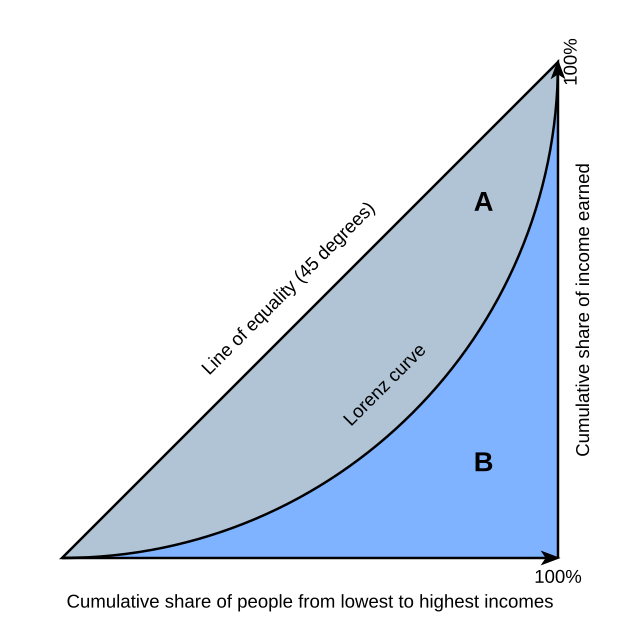
\includegraphics[width=0.6\textwidth]{pics/lfu2.png}
    \end{center} 

    \item Коэффициент Джини измеряет неравенство между значениями частотного распределения, такого как уровни дохода. Коэффициент Джини, равный 0, отражает идеальное равенство, когда все доходы или значения богатства одинаковы, в то время как коэффициент Джини, равный 1 (или 100\%), отражает максимальное неравенство между значениями, ситуацию, когда один человек имеет весь доход, а все остальные ничего не имеют.
\end{itemize}

Затем коэффициент Джини можно рассматривать как отношение площади, лежащей между линией равенства и кривой Лоренца (обозначенной как A на диаграмме), к общей площади под линией равенства (обозначенной как A и B на диаграмме); то есть G = A/(A + B). Он также равен 2А и 1 - 2В из-за того, что A + B = 0,5.

\subsection*{Алгебраическое представление. Доказательство линейной связи с AUC ROC}

\begin{itemize}
        \item ROC-кривая - это графическое представление того, как меняется доля истинно положительных предсказаний (TPR) в зависимости от доли ложно положительных предсказаний (FPR) порогового значения классификатора.

        \item Доля истинно положительных предсказаний (TPR), также известная как полнота, измеряет долю положительных образцов, которые правильно классифицируются как положительные.

        \item Доля ложно положительных предсказаний (FPR), также известная как частота ложных срабатываний, измеряет долю отрицательных образцов, которые неправильно классифицируются как положительные.

        \item AUC ROC – площадь под ROC-кривой – часто используют для оценивания качества упорядочивания алгоритмом объектов двух классов. Ясно, что это значение лежит на отрезке [0, 1]. 

        На самом деле же AUC ROC равен доле пар объектов вида (объект класса 1, объект класса 0), которые алгоритм верно упорядочил, т.е. первый объект идёт в упорядоченном списке раньше.
    \end{itemize}

Введём следующие обозначения:

$n$ — Количество объектов в выборке

$n_0$ — Количество объектов класса «0»

$n_1$ — Количество объектов класса «1»

$TP$ — True Positive (верный ответ модели на истинном классе «1» при заданном пороге)

$FP$ — False Positive (неверный ответ модели на истинном классе «0» при заданном пороге)

$TPR$ — True Positive Rate (отношение $TP$ к $n_1$)

$FPR$ — False Positive Rate (отношение $FP$ к $n_0$)

$i, j$ — текущий индекс элемента.


{\bf Параметрический метод}

Параметрическое уравнение для ROC curve можно записать в следующем виде:
$$AUC = \int_{0}^{1} TPR \enspace dFPR = \int_{0}^{1} \frac{TP}{n_1} \enspace d\frac{FP}{n_0} = \frac{1}{n_1*n_0}\int_{0}^{1}TP \enspace dFP $$


При построении графика Lift Curve по оси $X$ мы откладывали долю объектов (их количество) предварительно отсортированных по убыванию. Таким образом, параметрическое уравнение для Коэффициента Джини будет выглядеть следующим образом:

$$AUC = \int_{0}^{1} TPR \enspace d\frac{TP + FP}{n_1+n_0} - 0.5 $$



Подставив последнее выражение в желаемое и преобразовав его, мы увидим, что в одну из частей можно будет подставить предыдущее выражение, что в итоге даст нам красивую формулу нормализованного Джини
$$Gini_{normalized} = 2 * AUCROC - 1$$

{\bf Непараметрический метод}

Непараметрический метод основан на том, что AUC ROC равно статистике Вилкоксона-Манна-Уитни:

$$AUCROC = \frac{\sum_{i=1}^{n_1} \sum_{j=1}^{n_0} S(x_i, x_j)}{n_1*n_0} $$


\begin{center}
$S(x_i, x_j) = \begin{cases} 1, \enspace x_i > x_j\\ \frac{1}{2}, \enspace x_i = x_j \\ 0,\enspace x_i < x_j \end{cases}$
\end{center}


где $x_i$ — ответ алгоритма на i-ом объекте из распределения «1», $x_j$ — ответ алгоритма на j-ом объекте из распределения «0»

Интерпретируется это так: если случайным образом извлечь пару объектов, где первый объект будет из распределения «1», а второй из распределения «0», то вероятность того, что первый объект будет иметь предсказанное значение больше или равно, чем предсказанное значение второго объекта, равно значению AUC ROC. Комбинаторно несложно подсчитать, что количество пар таких объектов будет: $n_1*n_0$.


\subsection*{Задачи}

\begin{itemize}
    \item Рассмотрим простой случай где есть только два уровня дохода: низкий и высокий. Если группа с высоким доходом составляет часть u населения и зарабатывает часть f от общего дохода, то коэффициент Джини равен 
    $$S_{under} = \frac{(1-u)(1-f) + fu + 2u(1 - f)}{2} = \frac{1 - u - f + 2uf + 2u -2uf}{2} = \frac{1 + u - f}{2}$$
    $$S_{between} = 0.5 - \frac{1 + u - f}{2} = \frac{f - u}{2}$$
    $$Gini = \frac{\frac{f - u}{2}}{0.5} = f - u$$
    
    \begin{center}
        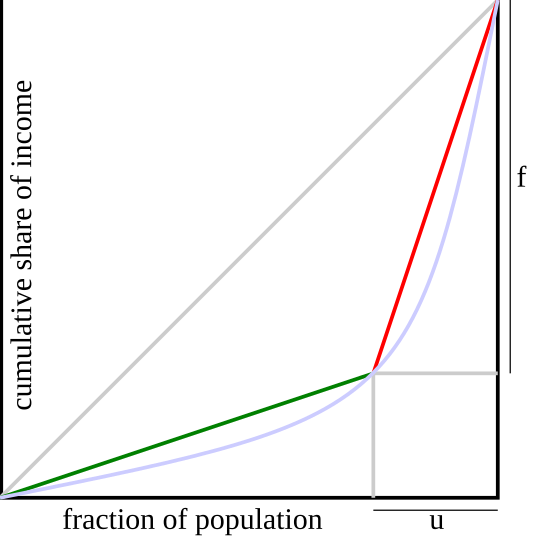
\includegraphics[width=0.6\textwidth]{pics/prim.png}
    \end{center} 

    \item Расммотрим еще один дискретный пример, где есть выборка из 10 человек, с соответствующими доходами $$[1, 1, 1, 3, 4, 7, 7, 10, 15, 20]$$

    Построим по ним кривую Лоренца, равенства и высчитаем индекс Джини


    \begin{center}
        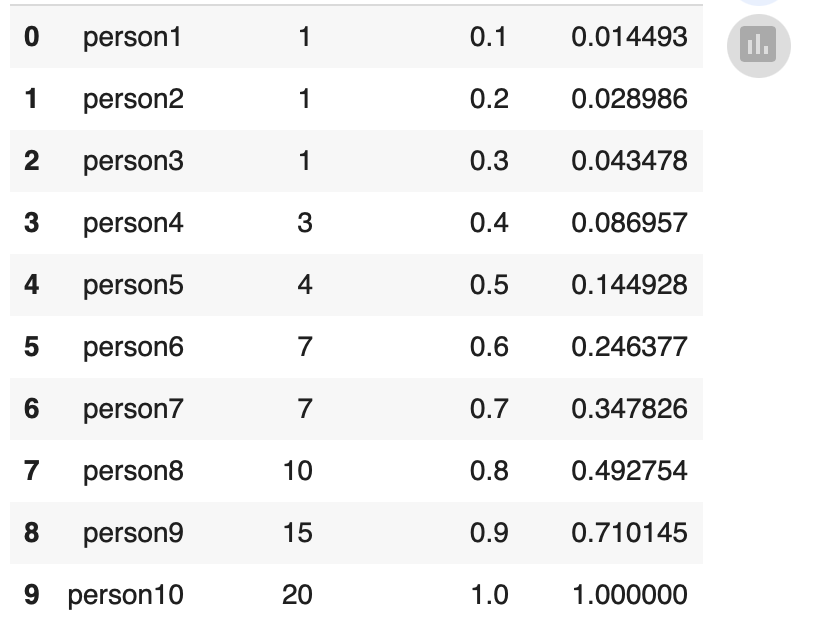
\includegraphics[width=0.6\textwidth]{pics/stolb.png}
    \end{center} 


    \begin{center}
        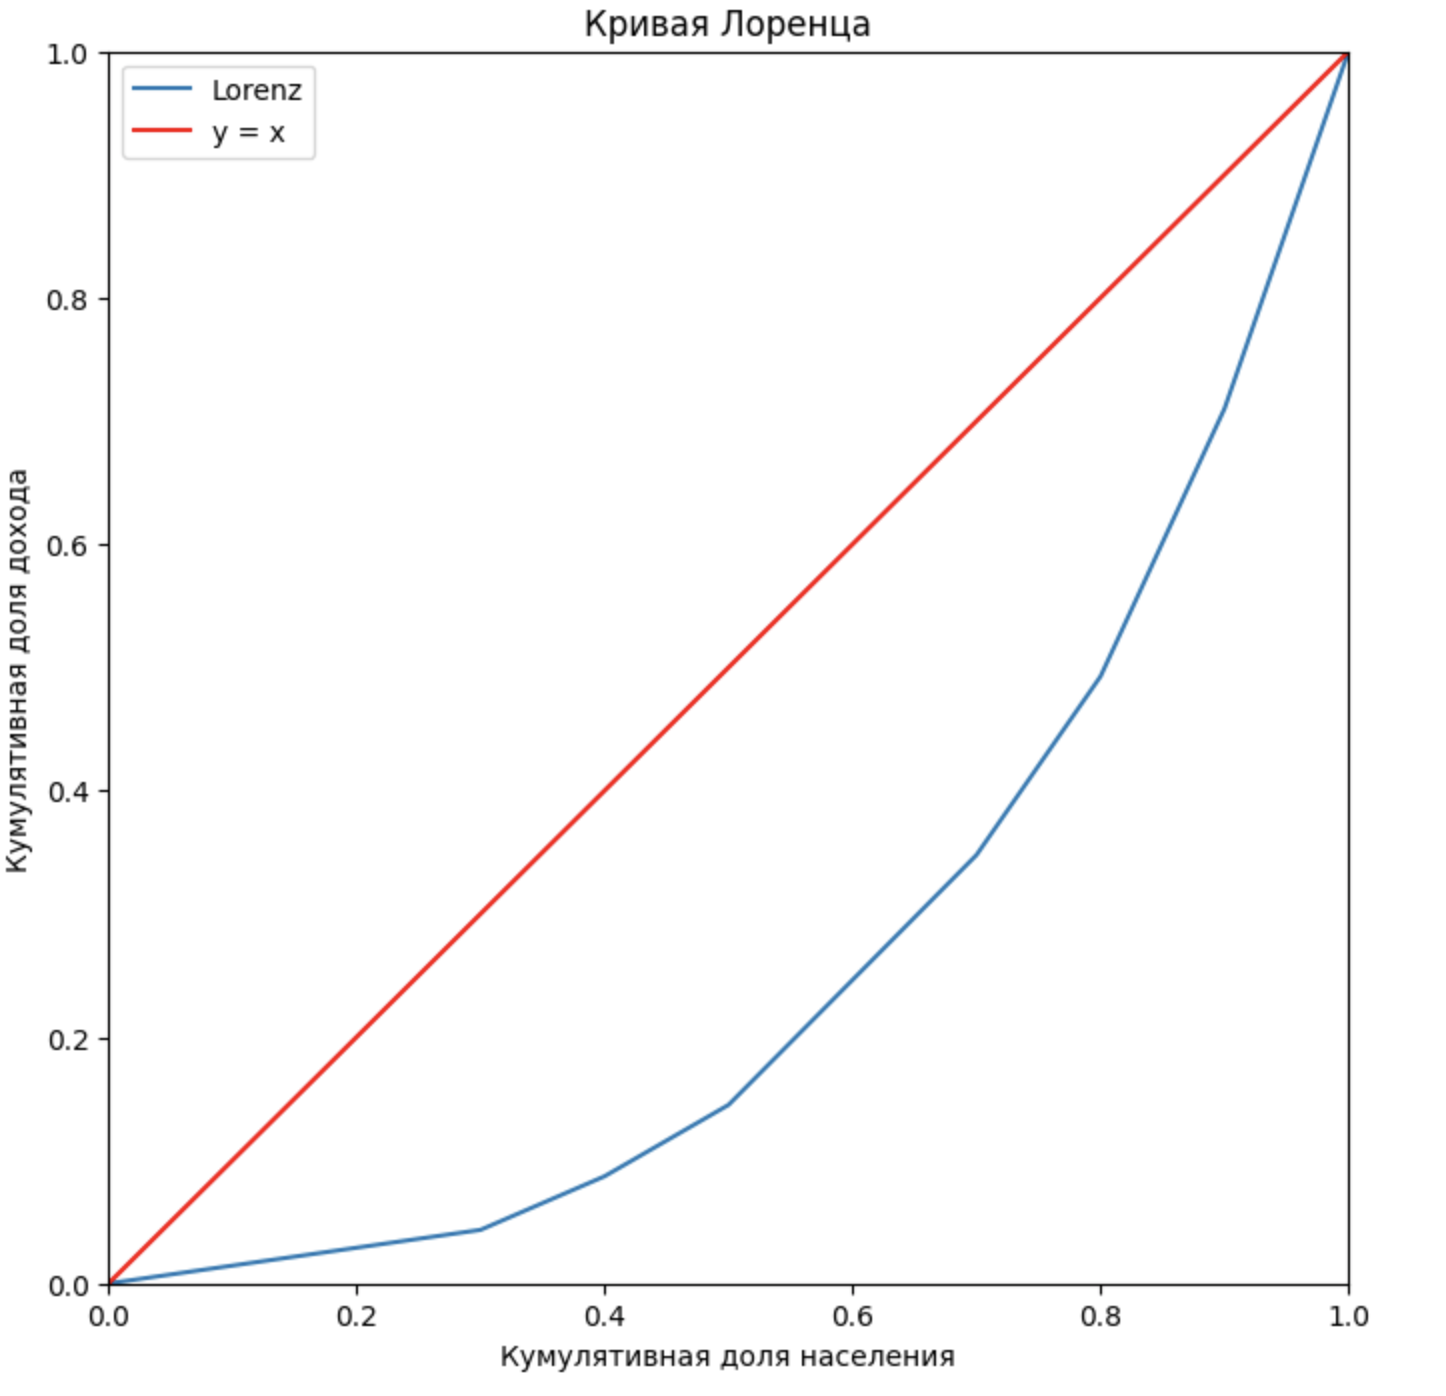
\includegraphics[width=0.6\textwidth]{pics/graph.png}
    \end{center} 

    \begin{center}
        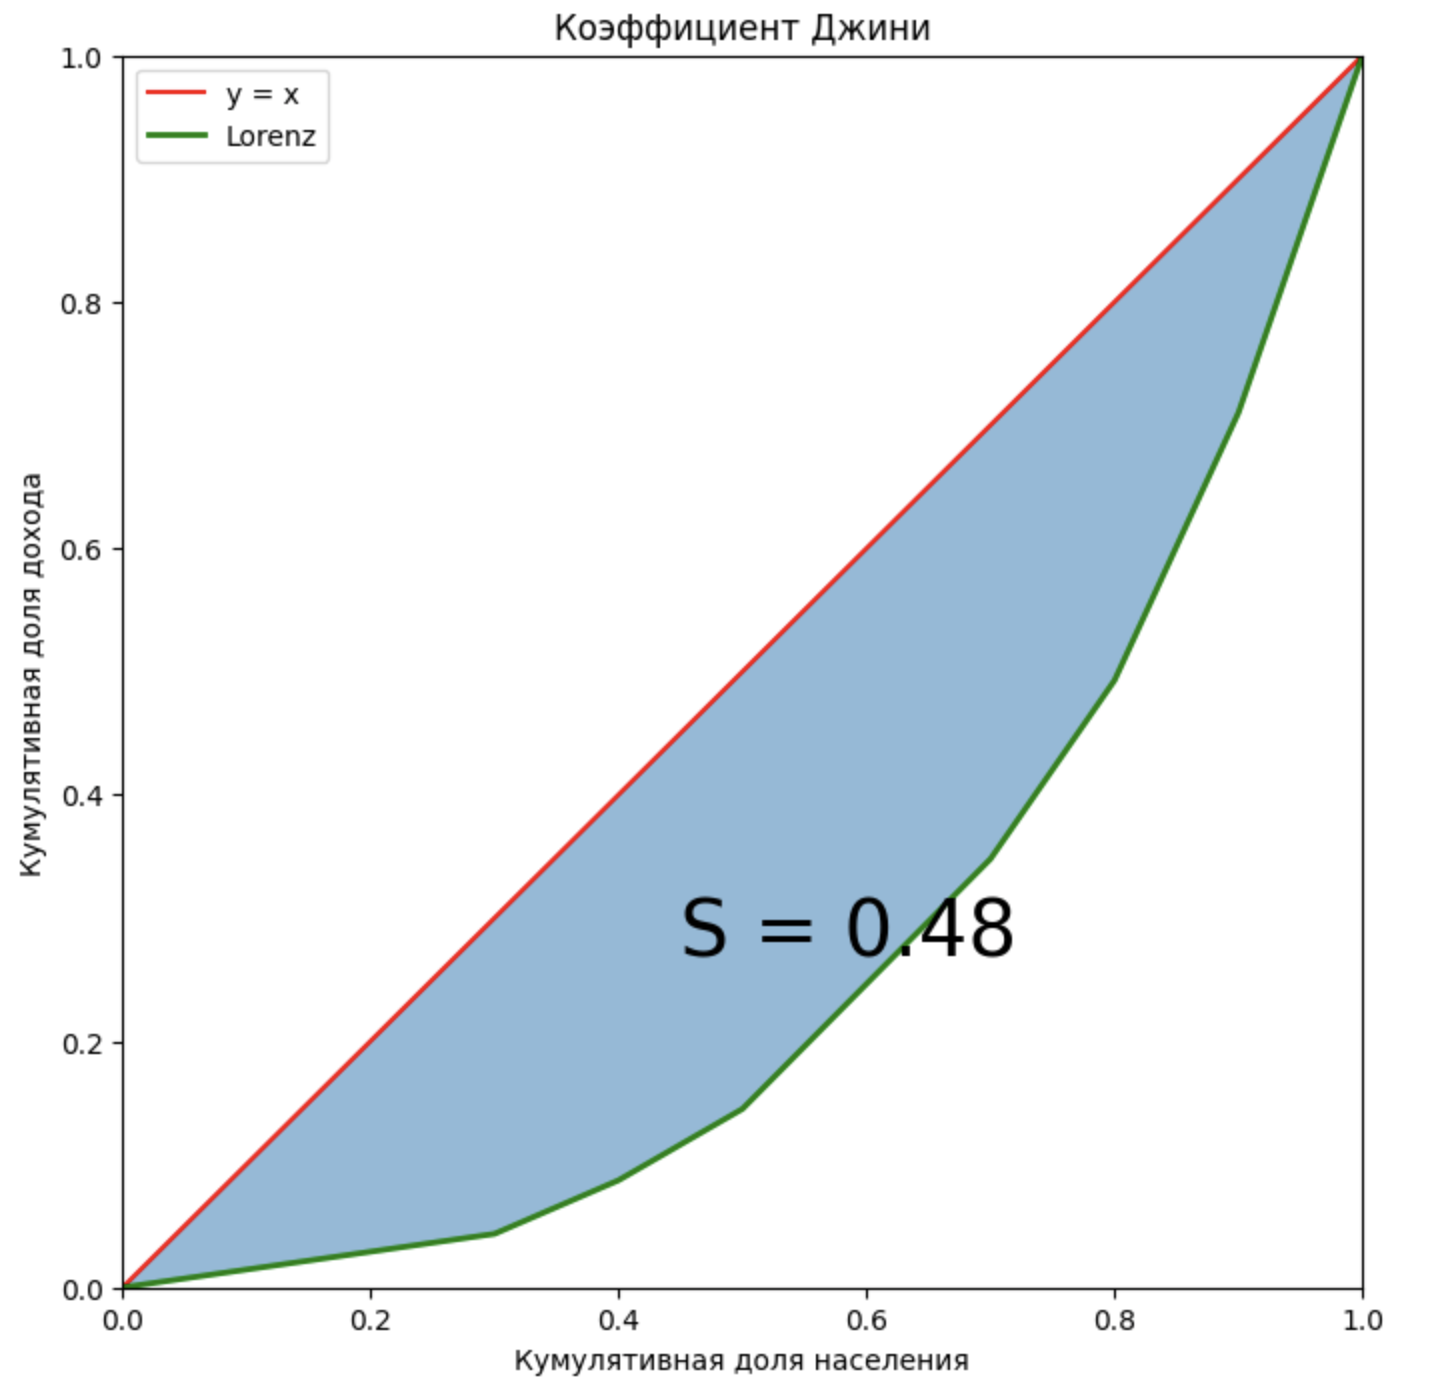
\includegraphics[width=0.6\textwidth]{pics/gini.png}
    \end{center} 

    Проделав то же самое для списка доходов $$[6, 7, 7, 7, 7, 7, 7, 7, 7, 7]$$ получим коэффицинт Джини равный $0.01$

    \begin{center}
        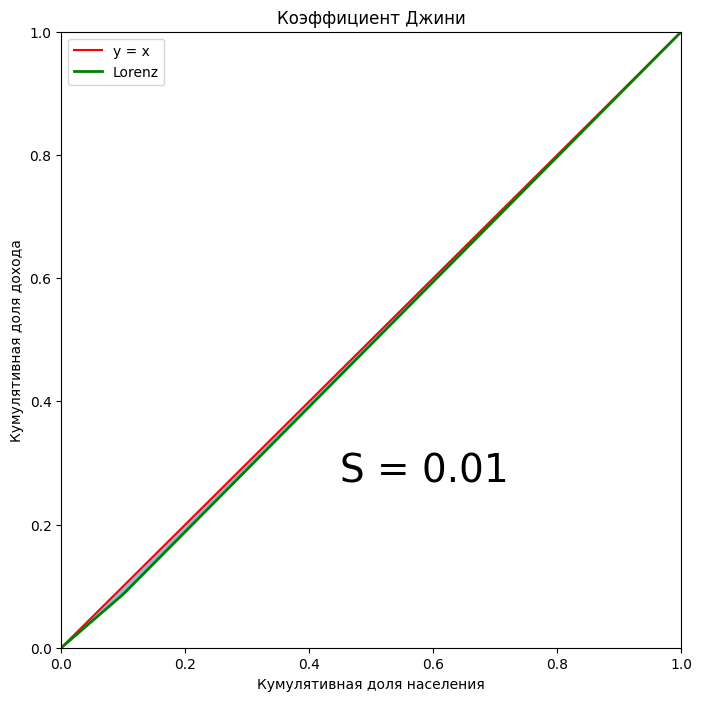
\includegraphics[width=0.6\textwidth]{pics/gini2.png}
    \end{center} 

    \item Коэффициент Джини также можно рассматривать как половину относительного среднего абсолютного отклонения. Для случайной выборки S со значениями $y_1 \leq y_2 \leq ... \leq y_n$

    $${\displaystyle G(S)={\frac {1}{n-1}}\left(n+1-2\left({\frac {\sum _{i=1}^{n}(n+1-i)y_{i}}{\sum _{i=1}^{n}y_{i}}}\right)\right)}$$

    упрощаем:

    $${\displaystyle G(S)=1-{\frac {2}{n-1}}\left(n-{\frac {\sum _{i=1}^{n}iy_{i}}{\sum _{i=1}^{n}y_{i}}}\right).}$$

    \item Метрикой качества в машинном обучении является нормализованный коэффициент Джини, который равен отношению коэффициента обученной модели к коэффициенту идеальной модели.
$$Gini_{normalized} = \frac{Gini_{model}}{Gini_{perfect}} $$
    Так сделано ввиду того, что "читсый" коэффициент Джини без знания точного значения коэффициента для идеального алгоритма не говорит нам ни о чем. 
    На самом деле, коэффициент Джини в машинном обучении хоть и близок к введенному нам экономическому, но высчитывается по формуле, описанной выше 
$$Gini_{normalized} = 2 * AUCROC - 1$$

\item {\bf Задача} 
Есть два набора данных:  

1. Набор A: классы 1, 1, 0, 1, 0  
2. Набор B: классы 1, 0, 0, 0, 0  

В каждом из наборов рассчитайте коэффициент Джини, показывающий степень однородности данных.  

Решение:  
Формула коэффициента Джини:  
$$[
Gini = 1 - \sum_{i=1}^{n} p_i^2
]  $$
где $(p_i)$ — доля объектов каждого класса.

Для набора A:  
- Класс 1: $(p_1 = \frac{3}{5})$  
- Класс 0: $(p_0 = \frac{2}{5})$

$$[
Gini_A = 1 - \left(\left(\frac{3}{5}\right)^2 + \left(\frac{2}{5}\right)^2\right) = 1 - \left(0.36 + 0.16\right) = 0.48
]$$

Для набора B:  
- Класс 1: $(p_1 = \frac{1}{5}) $
- Класс 0: $(p_0 = \frac{4}{5}) $

$$[
Gini_B = 1 - \left(\left(\frac{1}{5}\right)^2 + \left(\frac{4}{5}\right)^2\right) = 1 - \left(0.04 + 0.64\right) = 0.32
]$$

Ответ:  
- Gini для набора A = 0.48  
- Gini для набора B = 0.32  

Набор B однороднее, так как его коэффициент Джини ниже.

\end{itemize}

\subsection*{Отбор признаков с использованием индекса Джини}

Отбор признаков с использованием индекса Джини включает следующие шаги:

\begin{enumerate}
    \item Для каждого признака вычислить индекс Джини для всех возможных пороговых значений.
    \item Выбрать пороговое значение, которое дает наименьший индекс Джини.
    \item Разделить набор данных на два подмножества в зависимости от выбранного порогового значения.
\end{enumerate}


\subsection*{Преимущества}

\begin{enumerate}
    \item {\bf Вычислительная эффективност} Индекс Джини - это менее сложная и более быстрая в вычислениях мера по сравнению с другими мерами, такими как энтропия, которая включает вычисление логарифмов.
    \item {\bf Интуитивная интерпретация} Индекс Джини прост и удобен для интерпретации. Он измеряет вероятность того, что случайно выбранный образец из множества будет неверно классифицирован, если бы он был случайно помечен в соответствии с распределением классов во множестве.
    \item {\bf Хорошо подходит для бинарной классификации} Индекс Джини особенно эффективен для задач бинарной классификации, где целевая переменная имеет только два класса. В таких случаях известно, что индекс Джини более стабилен, чем другие меры.
\end{enumerate}


\subsection*{Недостатки}

\begin{enumerate}
 \item {\bf Недостатки AUC-ROC и Gini для несбалансированных выборок}
    Такие метрики, как accuracy и error rate, являются простыми интерпретируемыми метриками, однако они
    не подходят для оценки классификаторов, обученных на несбалансированных выборках. Например,
    если нам необходимо построить модель для выявления мошеннических кредитных заявок, доля которых
    составляет 1\% от всех заявок, тогда простой классификатор, относящий все кредитные заявки в класс «не мошеннические», будет иметь ассигасу = 99\% и error\_rate = 1\%, что является хорошими показателями качества. Однако такой классификатор будет бесполезен для бизнеса, поскольку он не выявляет ни одной мошеннической заявки.
    Такая же проблема возникает при использовании метрик AUC-ROC и Gini. Доказательство этого факта приводят в своем исследовании норвежские ученые Takaya Saito и Mark Rehmsmeie.
    Другим недостатком AUC-ROC, Gini является то, что эти метрики являются
    интегральными, то есть теряют часть информации. В результате может оказаться, что модели с
    одинаковыми значениями AUC-ROC будут работать по-разному.
    
    \begin{center}
        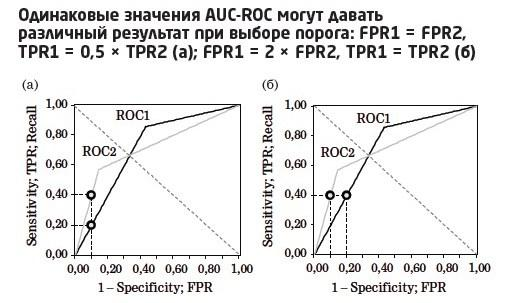
\includegraphics[width=0.6\textwidth]{pics/fff.jpeg}
    \end{center} 
    \item {\bf Не подходит для непрерывных переменных} Индекс Джини не подходит для непрерывных переменных, поскольку требует дискретизации переменной в категории или интервалы, что может привести к потере информации и снижению точности.
    \item {\bf Игнорирует взаимодействия между признаками} Индекс Джини учитывает только индивидуальную предсказательную силу каждого признака и игнорирует взаимодействия между признаками. Это может привести к неудачным разбиениям и менее точным прогнозам.
\end{enumerate}

\section*{Заключение}
Индекс Джини - это важная мера нечистоты, используемая в алгоритмах деревьев решений для задач классификации. Он измеряет вероятность того, что случайно выбранный экземпляр будет неправильно классифицирован алгоритмом дерева решений, и его значение варьируется от 0 (совершенно чистое) до 1 (совершенно нечистое). Индекс Джини прост в реализации, вычислительно эффективен и устойчив к выбросам. Он был использован в различных приложениях машинного обучения, таких как обнаружение мошенничества, оценка кредитоспособности и сегментация клиентов.

\end{document}
